\documentclass[12pt,a4paper]{article}

% ─── Page Layout ───────────────────────────────────────────────────────────────
\usepackage[a4paper, margin=0.8in, headheight=14pt]{geometry}

% ─── Fonts (XeLaTeX) ───────────────────────────────────────────────────────────
\usepackage{fontspec}
\usepackage{unicode-math}
\setmainfont{TeX Gyre Pagella}
\setmonofont[Scale=0.88]{TeX Gyre Cursor}
\setmathfont{Latin Modern Math}

% ─── Packages ──────────────────────────────────────────────────────────────────
\usepackage{xcolor}
\usepackage{colortbl}
\usepackage{titlesec}
\usepackage{enumitem}
\usepackage{tabularx}
\usepackage{booktabs}
\usepackage{array}
\usepackage{amsmath}
\usepackage{tikz}
\usetikzlibrary{shapes.geometric, arrows.meta, positioning, calc, fit, decorations.pathreplacing}
\usepackage{tcolorbox}
\tcbuselibrary{skins, breakable}
\usepackage{hyperref}
\usepackage{fancyhdr}
\usepackage{graphicx}
\usepackage{microtype}
\hyphenpenalty=10000
\exhyphenpenalty=10000
\sloppy
\usepackage{caption}
\usepackage{setspace}
\usepackage{multirow}
\usepackage{tocloft}

% ─── Q&A helper ────────────────────────────────────────────────────────────────
\newcommand{\Q}[1]{\textbf{#1}\par\noindent\ignorespaces}

% ─── Colour Palette ────────────────────────────────────────────────────────────
\definecolor{myred}{RGB}{196,30,58}
\definecolor{mydark}{RGB}{30,30,50}
\definecolor{mygreen}{RGB}{14,120,80}
\definecolor{myteal}{RGB}{0,130,140}
\definecolor{myamber}{RGB}{180,100,0}
\definecolor{mypurple}{RGB}{100,30,160}
\definecolor{mygray}{RGB}{246,247,249}
\definecolor{mgframe}{RGB}{180,185,200}
\definecolor{watermark}{RGB}{145,150,170}
\definecolor{hdrred}{RGB}{250,232,235}
\definecolor{hdrgreen}{RGB}{220,244,233}
\definecolor{hdrteal}{RGB}{220,242,244}
\definecolor{hdramber}{RGB}{253,242,215}
\definecolor{hdrpurple}{RGB}{238,228,255}
\definecolor{hdrgray}{RGB}{238,240,245}
\definecolor{rowalt}{RGB}{250,251,253}

% ─── Section Formatting ────────────────────────────────────────────────────────
\titleformat{\section}
  {\large\bfseries\color{myred}}{\thesection.}{0.5em}{}
  [\vspace{1pt}{\color{myred}\rule{\linewidth}{0.8pt}}]
\titleformat{\subsection}
  {\normalsize\bfseries\color{myteal}}{\thesubsection}{0.5em}{}
\titlespacing*{\section}{0pt}{18pt}{7pt}
\titlespacing*{\subsection}{0pt}{11pt}{4pt}

% ─── Paragraph ─────────────────────────────────────────────────────────────────
\setlength{\parindent}{0pt}
\setlength{\parskip}{4pt}

% ─── TOC Styling ───────────────────────────────────────────────────────────────
\renewcommand{\cfttoctitlefont}{\large\bfseries\color{myred}}
\renewcommand{\cftaftertoctitle}{\par\noindent{\color{myred}\rule{\linewidth}{0.8pt}}}
\setlength{\cftbeforetoctitleskip}{0pt}
\setlength{\cftaftertoctitleskip}{6pt}
\renewcommand{\cftsecfont}{\normalsize\bfseries\color{mydark}}
\renewcommand{\cftsecpagefont}{\normalsize\bfseries\color{mydark}}
\renewcommand{\cftsecleader}{\cftdotfill{\cftdotsep}}
\setlength{\cftbeforesecskip}{7pt}
\renewcommand{\cftsubsecfont}{\small\color{mydark}}
\renewcommand{\cftsubsecpagefont}{\small\color{mydark}}
\setlength{\cftbeforesubsecskip}{3pt}
\setlength{\cftsubsecindent}{1.4em}

% ─── Table helpers ─────────────────────────────────────────────────────────────
\renewcommand{\arraystretch}{1.45}
\setlength{\tabcolsep}{6pt}
\arrayrulecolor{mydark}
\newcolumntype{B}[1]{>{\small\bfseries\raggedright\arraybackslash}m{#1}}
\newcolumntype{Y}{>{\small\raggedright\arraybackslash}X}
\renewcommand{\tabularxcolumn}[1]{m{#1}}

% ─── Header / Footer ───────────────────────────────────────────────────────────
\pagestyle{fancy}
\fancyhf{}
\fancyhead[L]{\small\color{myred}\textbf{OE-EC604B}\;\color{mydark}--- Operating System}
\fancyhead[R]{\small\color{myteal}\textbf{Module 2 Notes}}
\fancyfoot[C]{\small\color{mydark}\thepage}
\fancyfoot[R]{\small\color{watermark}\textit{\copyright\ Biraj}}
\renewcommand{\headrulewidth}{0.5pt}
\renewcommand{\footrulewidth}{0.3pt}

% ─── Hyperref ──────────────────────────────────────────────────────────────────
\hypersetup{
  colorlinks=true, linkcolor=myteal, urlcolor=myteal,
  pdfauthor={Biraj Sarkar},
  pdftitle={OE-EC604B --- Module 2 Notes}
}

% ─── tcolorbox styles ──────────────────────────────────────────────────────────
\tcbset{
  tikzbox/.style={
    colback=mygray, colframe=mgframe, boxrule=0.6pt, arc=4pt,
    left=8pt, right=8pt, top=6pt, bottom=6pt,
    colbacktitle=mgframe, coltitle=mydark,
    fonttitle=\small\bfseries
  },
  defbox/.style={
    colback=hdrgreen, colframe=mygreen, boxrule=0.8pt, arc=4pt,
    left=9pt, right=9pt, top=6pt, bottom=6pt,
    colbacktitle=mygreen, coltitle=white,
    fonttitle=\small\bfseries
  },
  formulabox/.style={
    colback=hdrteal, colframe=myteal, boxrule=0.8pt, arc=4pt,
    left=9pt, right=9pt, top=7pt, bottom=7pt,
    colbacktitle=myteal, coltitle=white,
    fonttitle=\small\bfseries
  },
  examplebox/.style={
    colback=hdramber, colframe=myamber, boxrule=0.8pt, arc=4pt,
    left=9pt, right=9pt, top=6pt, bottom=6pt,
    colbacktitle=myamber, coltitle=white,
    fonttitle=\small\bfseries
  },
  masonbox/.style={
    colback=hdrpurple, colframe=mypurple, boxrule=0.8pt, arc=4pt,
    left=9pt, right=9pt, top=6pt, bottom=6pt,
    colbacktitle=mypurple, coltitle=white,
    fonttitle=\small\bfseries
  },
  exambox/.style={
    colback=hdrpurple, colframe=mypurple, boxrule=1pt, arc=5pt,
    left=10pt, right=10pt, top=8pt, bottom=8pt,
    colbacktitle=mypurple, coltitle=white,
    fonttitle=\bfseries,
    breakable, title after break={\textbf{Frequently Asked / Viva Questions (contd.)}}}
}
% Make all boxes breakable across pages
\tcbset{breakable}

% ─── TikZ styles ───────────────────────────────────────────────────────────────
\tikzset{
  block/.style={rectangle, draw=myteal, fill=hdrteal,
    text width=2.4cm, align=center, minimum height=0.95cm,
    font=\small, rounded corners=3pt, line width=0.7pt},
  redblock/.style={rectangle, draw=myred, fill=hdrred,
    text width=2.4cm, align=center, minimum height=0.95cm,
    font=\small, rounded corners=3pt, line width=0.7pt},
  greenblock/.style={rectangle, draw=mygreen, fill=hdrgreen,
    text width=2.4cm, align=center, minimum height=0.95cm,
    font=\small, rounded corners=3pt, line width=0.7pt},
  amberblock/.style={rectangle, draw=myamber, fill=hdramber,
    text width=2.4cm, align=center, minimum height=0.95cm,
    font=\small, rounded corners=3pt, line width=0.7pt},
  purpblock/.style={rectangle, draw=mypurple, fill=hdrpurple,
    text width=2.4cm, align=center, minimum height=0.95cm,
    font=\small, rounded corners=3pt, line width=0.7pt},
  sumjunc/.style={circle, draw=myamber, fill=hdramber,
    minimum size=0.62cm, font=\small, line width=0.8pt},
  arrow/.style={-Stealth, thick, color=mydark},
  redarrow/.style={-Stealth, thick, color=myred},
  line/.style={thick, color=mydark}
}

% ═══════════════════════════════════════════════════════════════════════════════
\begin{document}
% ═══════════════════════════════════════════════════════════════════════════════

\begin{center}
  {\LARGE\bfseries\color{myred} OE-EC604B --- Operating System}\\[5pt]
  {\normalsize\color{mydark} Semester VI \quad$\bullet$\quad 3L:0T:0P \quad$\bullet$\quad 3 Credits}\\[3pt]
  {\normalsize\color{myteal}\textbf{Module 2 Exam Notes: Operating System Structures}}\\[3pt]
  {\small\color{mydark} CGEC \;$|$\; B.Tech ECE (2023--27) \;$|$\; \textit{Biraj Sarkar}}
\end{center}
\vspace{2pt}
\noindent{\color{myred}\rule{\linewidth}{1.5pt}}
\vspace{2pt}

\hypersetup{linkcolor=mydark}
\tableofcontents
\hypersetup{linkcolor=myteal}
\newpage

% ===============================================================================
\section{System Components and Operating System Services}
% ===============================================================================

An operating system provides an environment for the execution of programs by presenting services to both users and system processes.

\subsection{Operating System Services}
The OS provides services that make computer usage convenient and efficient:
1. \textbf{User Interface (UI):} Command Line Interface (CLI), Graphics User Interface (GUI), or Batch Interface.
2. \textbf{Program Execution:} Loading a program into memory, executing it, and terminating it (either normally or abnormally).
3. \textbf{I/O Operations:} Managing read/write transfers to files or hardware devices since user programs cannot access hardware directly.
4. \textbf{File-System Manipulation:} Creating, deleting, searching, reading, writing, and controlling file access permissions.
5. \textbf{Communications:} Exchanging information between processes running on the same computer or different machines via networks (using shared memory or message passing).
6. \textbf{Error Detection:} Continuously monitoring for hardware errors (memory parity, power failure) or software errors (arithmetic overflow, illegal memory access) and executing handling procedures.
7. \textbf{Resource Allocation:} Distributing CPU cycles, main memory, and file storage dynamically among active users or jobs.
8. \textbf{Accounting:} Tracking user resource usage for billing, statistics, or system profiling.
9. \textbf{Protection \& Security:} Controlling access to system resources and securing user authentication.

\subsection{System Calls}

\begin{tcolorbox}[defbox, title={\textbf{Definition: System Call}}]
A \textbf{System Call} is the programmatic interface that allows a running program (in user space) to request services directly from the operating system kernel (in kernel space).
\end{tcolorbox}

\begin{itemize}[leftmargin=*, itemsep=3pt]
  \item \textbf{Dual-Mode Operation:} Modern hardware supports at least two modes of operation: \textbf{User Mode (mode bit = 1)} and \textbf{Kernel/Supervisor Mode (mode bit = 0)}. System calls trigger a software interrupt (trap instruction) that shifts execution from user mode to kernel mode to run privileged instructions.
\end{itemize}

\begin{tcolorbox}[tikzbox, title={System Call Execution Flow}]
\centering
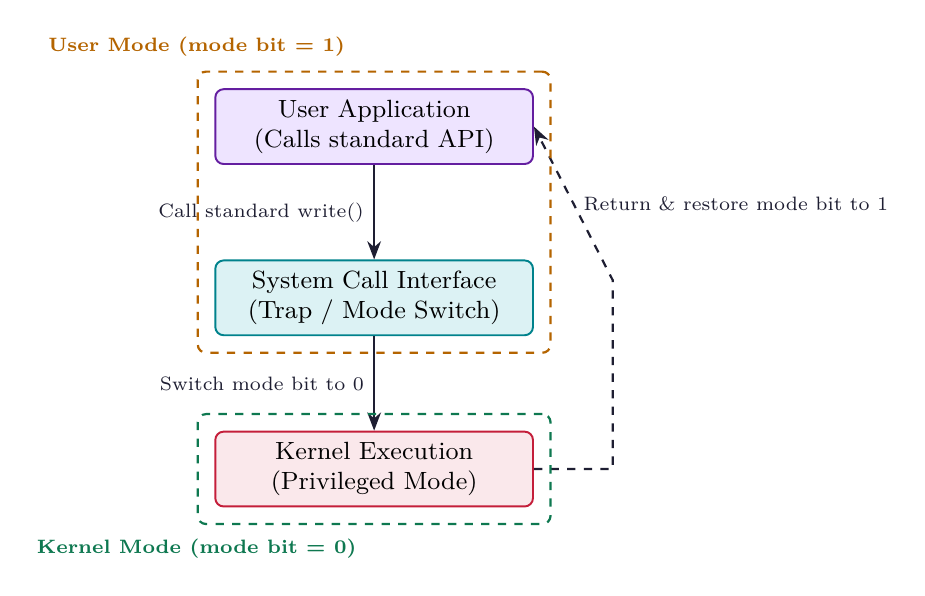
\begin{tikzpicture}[node distance=1.1cm and 2.5cm, thick, font=\small]
  \node[block, text width=3.8cm, fill=hdrpurple, draw=mypurple] (userprog) {User Application\\(Calls standard API)};
  \node[block, text width=3.8cm, fill=hdrteal, draw=myteal, below=1.2cm of userprog] (syscall) {System Call Interface\\(Trap / Mode Switch)};
  \node[block, text width=3.8cm, fill=hdrred, draw=myred, below=1.2cm of syscall] (kernel) {Kernel Execution\\(Privileged Mode)};

  \draw[arrow] (userprog.south) -- node[left, font=\scriptsize] {Call standard write()} (syscall.north);
  \draw[arrow] (syscall.south) -- node[left, font=\scriptsize] {Switch mode bit to 0} (kernel.north);
  \draw[arrow, dashed] (kernel.east) -- ++(1.0, 0) -- ++(0, 2.4) -- node[right, font=\scriptsize] {Return \& restore mode bit to 1} (userprog.east);

  \node[draw=myamber, dashed, inner sep=6pt, rounded corners=3pt, fit=(userprog) (syscall)] (usermode) {};
  \node[font=\scriptsize\bfseries\color{myamber}, above=0.05cm of usermode.north west] {User Mode (mode bit = 1)};
  \node[draw=mygreen, dashed, inner sep=6pt, rounded corners=3pt, fit=(kernel)] (kernelmode) {};
  \node[font=\scriptsize\bfseries\color{mygreen}, below=0.05cm of kernelmode.south west] {Kernel Mode (mode bit = 0)};
\end{tikzpicture}
\end{tcolorbox}

% ===============================================================================
\section{Operating System Architecture Structures}
% ===============================================================================

Operating systems must be structured to ensure reliability, performance, and ease of modification. There are four traditional design methodologies:

\subsection{Monolithic Structure}
In a monolithic operating system, all OS code (scheduling, filesystem, memory management, drivers) runs in a single address space in kernel mode.
\begin{itemize}[leftmargin=*, itemsep=3pt]
  \item \textbf{Advantages:} High performance due to minimal context switching overhead.
  \item \textbf{Disadvantages:} Lack of safety --- a bug in any module (like a camera driver) can crash the entire system.
\end{itemize}

\subsection{Layered Structure}
The OS is broken into a hierarchy of layers (0 to N). Layer 0 is the hardware; Layer N is the user interface.
\begin{itemize}[leftmargin=*, itemsep=3pt]
  \item \textbf{Design Rule:} Each layer is built upon and can only invoke services of lower-level layers.
  \item \textbf{Advantages:} Modular development, simplified debugging.
  \item \textbf{Disadvantages:} Hard to define layers cleanly, and poor performance because each layer crossing introduces execution overhead.
\end{itemize}

\subsection{Microkernel Structure}
The microkernel architecture structures the OS by removing all non-essential components from the kernel, implementing them instead as user-space programs (servers).
\begin{itemize}[leftmargin=*, itemsep=3pt]
  \item \textbf{Core Kernel Services:} Low-level memory management, thread scheduling, and Inter-Process Communication (IPC).
  \item \textbf{Advantages:} High security and reliability. If a filesystem service crashes, the rest of the OS remains unaffected.
  \item \textbf{Disadvantages:} High performance overhead because client programs must communicate with user-space servers via message passing, which requires frequent context switches.
\end{itemize}

\subsection{Hybrid Systems}
Most modern operating systems (e.g., Windows NT, macOS, Linux) use a hybrid design. They combine monolithic speed with microkernel modularity, running core modules in a single address space while using dynamic modules (loadable kernel modules) for extensibility.

\newpage
% ===============================================================================
% MANDATORY QUICK REVISION PAGE
% ===============================================================================
\begin{center}
  {\large\bfseries\color{myred} Quick Revision --- Module 2}\\[3pt]
  {\small\color{mydark} Operating System Structures $|$ OE-EC604B}
\end{center}
\noindent{\color{myred}\rule{\linewidth}{1.2pt}}
\vspace{4pt}

\begin{tcolorbox}[formulabox, title={\textbf{System Call Parameter Passing Methods}}]
\renewcommand{\arraystretch}{1.3}
\begin{tabularx}{\linewidth}{B{3.5cm} X}
Register Method & Parameters passed directly in CPU registers. Fastest, but limited parameter capacity. \\[4pt]
Block / Table Method & Parameters written to a block in memory; pointer to the block is passed in a register. Unlimited size. \\[4pt]
Stack Method & Parameters pushed onto the user stack and popped off by the kernel. Unlimited size.
\end{tabularx}
\tcbset{breakable}
\end{tcolorbox}

\begin{tcolorbox}[defbox, title={\textbf{One-Line Definitions}}]
\begin{itemize}[leftmargin=*, itemsep=2.5pt, topsep=0pt]
  \item \textbf{System Call:} Programmatic request by user-mode applications to execute kernel-mode services.
  \item \textbf{Mode Bit:} A hardware register flag indicating User Mode (1) or Kernel Mode (0).
  \item \textbf{Monolithic Kernel:} OS design where all services run in a single address space inside kernel mode.
  \item \textbf{Microkernel:} Minimalist kernel executing only IPC, scheduling, and basic memory management.
  \item \textbf{Layered Architecture:} Hierarchy of OS layers where layer $i$ relies only on services of layer $i-1$.
  \item \textbf{Trap:} A software-generated interrupt caused by an error or system call request.
  \item \textbf{API (Application Programming Interface):} Standard set of functions wrapper around system calls (e.g., Win32, POSIX).
  \item \textbf{System Program:} File utilities, compilers, or editors that provide a shell wrapper around system calls.
\end{itemize}
\end{tcolorbox}

\begin{tcolorbox}[exambox, title={\textbf{Frequently Asked / Viva Questions}}]
\begin{enumerate}[topsep=0pt, label=\textbf{Q\arabic*.}, itemsep=5pt]
  \item \Q{Why is dual-mode operation supported by hardware in modern operating systems?}
    To protect the system from malicious or poorly written user applications. Privileged instructions (like I/O control or memory protection access) can only be executed in Kernel Mode.
  \item \Q{Describe the sequence of actions that occur when a system call is made.}
    The user program invokes the API function $\to$ API puts system call number in a register $\to$ triggers software interrupt (trap) $\to$ hardware switches mode bit to 0 $\to$ execution jumps to system call handler in kernel $\to$ handler executes kernel code $\to$ mode bit is reset to 1 $\to$ control returns to user program.
  \item \Q{Compare Monolithic Kernels and Microkernels in terms of reliability and performance.}
    Monolithic: High performance (fast function calls, no IPC overhead) but low reliability (any driver crash can bring down the entire OS). Microkernel: High reliability (isolated user-space services) but slower performance (heavy IPC message passing and context switches).
  \item \Q{What are system programs? Give two examples.}
    System programs are user-space utilities that provide a convenient environment for program development and execution. Examples: file command programs (\texttt{cp}, \texttt{mv}) and status utilities (\texttt{ps}, \texttt{top}).
  \item \Q{What are the three common methods used to pass parameters to the operating system during a system call?}
    1. Pass parameters in CPU registers. 2. Store parameters in a memory block/table and pass the block address in a register. 3. Push parameters onto the system stack.
  \item \Q{What is the difference between a system call and a library function?}
    A system call is handled directly by the kernel and involves context switching and privilege escalation. A library function (like \texttt{strlen()}) executes entirely in user mode without kernel intervention.
  \item \Q{Explain the concept of device drivers in OS structure.}
    Device drivers are specialized software modules that translate general I/O commands from the OS kernel into device-specific commands that can be interpreted by hardware controllers.
  \item \Q{Why does the layered architecture model suffer from performance issues?}
    Each layer boundary requires crossing and parameter validation. An application requesting a file read might have to traverse multiple layers sequentially, incurring cumulative overhead.
  \item \Q{What is the POSIX standard?}
    Portable Operating System Interface; a family of standards specified by the IEEE to clarify API compatibility between UNIX-like operating systems.
  \item \Q{How does a hybrid operating system achieve both reliability and speed?}
    By using a monolithic core for speed (running speed-critical elements like graphics and file systems in kernel space) but supporting dynamic loadable kernel modules (LKMs) for driver modularity.
\end{enumerate}
\end{tcolorbox}

\begin{tcolorbox}[tikzbox, title={Comparison of OS Architectures}]
\renewcommand{\arraystretch}{1.4}
\par\noindent
\begin{tabularx}{\linewidth}{|B{2.2cm}|>{\small\centering\arraybackslash}X|>{\small\centering\arraybackslash}X|>{\small\centering\arraybackslash}X|}
\hline
\textbf{Architecture} & \textbf{\color{myred}Context Switch Cost} & \textbf{\color{myteal}Reliability} & \textbf{\color{myamber}Extensibility} \\
\hline
\textbf{Monolithic} & Extremely Low (no IPC) & Poor (no protection) & Hard (requires recompile) \\
\hline
\textbf{Layered} & High (traverses layers) & Moderate & Moderate \\
\hline
\textbf{Microkernel} & Very High (heavy IPC) & Excellent & Very Easy (add user servers) \\
\hline
\end{tabularx}
\end{tcolorbox}

\end{document}
